\documentclass[11pt]{report}
\usepackage[margin=2cm]{geometry}
\usepackage{graphicx}
\usepackage{hyperref}
\usepackage{xspace}
\usepackage{caption}

\usepackage{float}
\usepackage{times}
\usepackage[dvipsnames]{xcolor}

\newcommand{\Gap}{\texorpdfstring{\hfill}{}}
\newcommand{\Rec}{\texorpdfstring{{\small\emph{\color{blue}{\fbox{High Leverage}}}}}{}}
\newcommand{\HighRisk}{\texorpdfstring{{\small\emph{\color{orange}{\fbox{Uncertain Impact}}}}}{}}
\newcommand{\Longterm}{\texorpdfstring{{\small\emph{\color{OliveGreen}{\fbox{Long-term}}}}}{}}

\newcommand{\cd}{CO$_2$\xspace}

\begin{document}
\section{Farms \& Forests\texorpdfstring{\hfill\textit{by Alexandre Lacoste}}{}} \label{sec:afolu}
Plants, microbes, and other organisms have been drawing \cd from the atmosphere for millions of years. Most of this carbon is continually broken down and recirculated through the carbon cycle, and some is stored deep underground as coal and oil, but a large amount of carbon is sequestered in the biomass of trees, peat bogs, and soil. Our current economy encourages practices that are freeing much of this sequestered carbon through deforestation and unsustainable agriculture. On top of these effects, cattle and rice farming generate methane, a greenhouse gas far more potent than \cd itself. Overall, land use by humans is estimated to be responsible for about a quarter of global GHG emissions \cite{ipcc2014summary} (and this may be an underestimate \cite{mahowald2017impacts}). In addition to this direct release of carbon through human actions, the permafrost is now melting, peat bogs are drying, and forest fires are becoming more frequent as a consequence of climate change itself -- all of which release yet more carbon \cite{Climate_change_feedback}.

The large scale of this problem allows for a similar scale of positive impact. According to one estimate \cite{hawken2017drawdown}, about a third of GHG emissions reductions could come from better land management and agriculture. ML can play an important role in some of these areas. Precision agriculture could reduce carbon release from the soil and improve crop yield, which in turn could reduce the need for deforestation. Satellite images make it possible to estimate the amount of carbon sequestered in a given area of land, as well as track GHG emissions from it. ML can help monitor the health of forests and peatlands, predict the risk of fire, and contribute to sustainable forestry (Fig.~\ref{fig:agriculture}). These areas represent highly impactful applications, in particular, of sophisticated computer vision tools, though care must be taken in some cases to avoid negative consequences via the Jevons paradox.

\begin{figure}[hbpt]
    \centering
    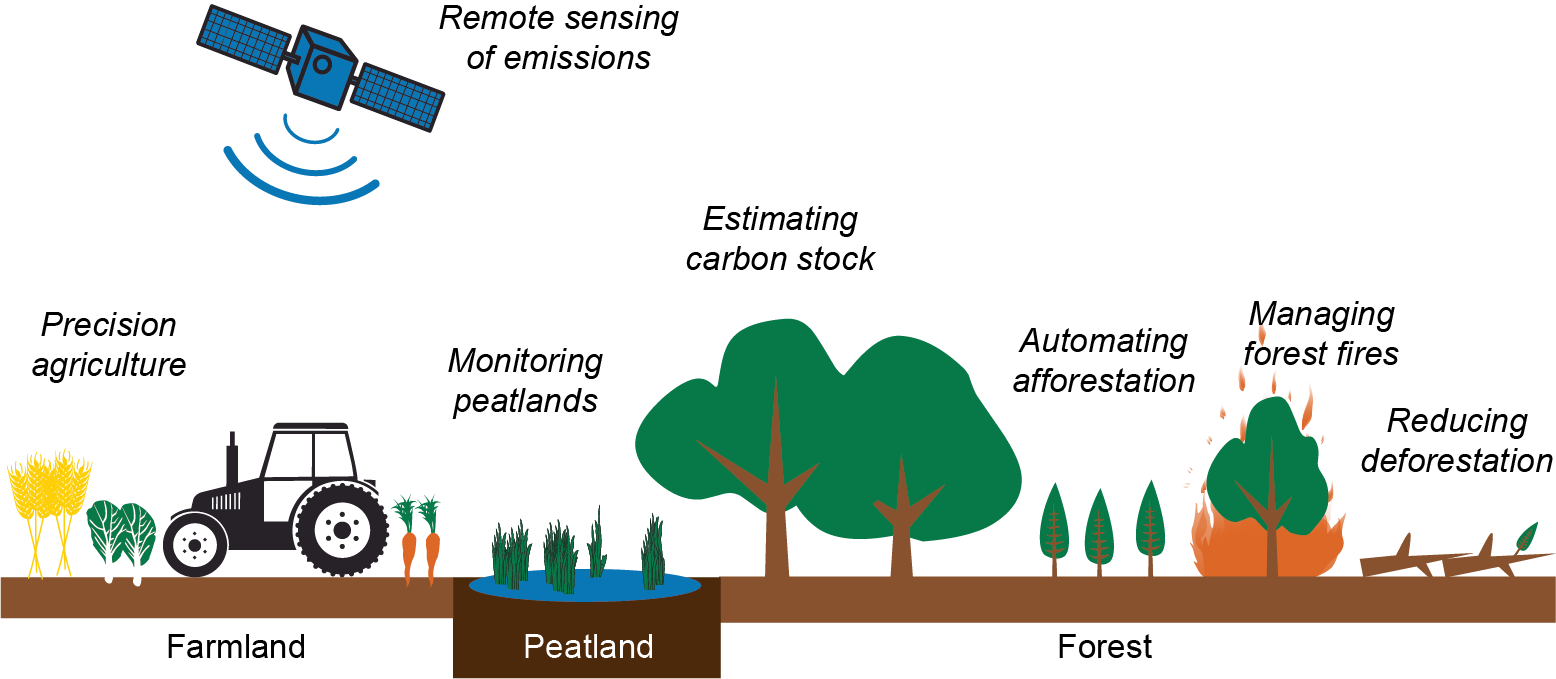
\includegraphics{figures/new_agriculture.png}
    \caption{Selected strategies to mitigate GHG emissions from land use using machine learning.}
    \label{fig:agriculture}
\end{figure}

\subsection{Remote sensing of emissions\Gap \Rec} \label{sec:emissions-detection}
Having real-time maps of GHGs could help us quantify emissions from agriculture and forestry practices, as well as monitor emissions from other sectors (\S \ref{sec:electricity-currentSystemImpact}).
 
Such information would be valuable in guiding regulations or incentives that could lead to better land use practices. For example, data on emissions make it possible to set effective targets, and pinpointing the sources of emissions makes it possible to enforce regulations.

While greenhouse gases are invisible to our eyes, they must by definition interact with sunlight. This means that we can observe these compounds with hyperspectral cameras \cite{Hyperspectral, scafutto2018detection}. These cameras can record up to several hundred wavelengths (instead of simply RGB), providing information on the interaction between light and individual chemicals. Many satellites are equipped with such cameras and can perform, to some extent, estimations of \cd, CH$_4$ (methane), H$_2$O, and N$_2$O (nitrous oxide) emissions \cite{jacob2016satellite, bernath2017near}. While extremely useful for studying climate change, most of these satellites have very coarse spatial resolution and large temporal and spatial gaps, making them unsuitable for precise tracking of emissions. Standard satellite imagery provides RGB images with much higher resolution, which could be used in an ML algorithm to fill the gaps in hyperspectral data and obtain more precise information about emissions\footnote{Microsatellites with higher resolution hyperspectral cameras are expected to launch over the coming years, including a proposal by Bluefield Technologies that would provide methane detection at 20-meter spatial resolution with daily refresh. Even once this technology comes online, ML will remain useful to cover the daily gaps and to estimate emissions of other GHGs.}. Some preliminary work \cite{jacob2016satellite} has studied this possibility, but there are no clear results as of yet. This is therefore an open problem with high potential impact.

\subsection{Precision agriculture\Gap \Rec
\HighRisk}\label{sec:agriculture}
Agriculture is responsible for about 14\% of GHG emissions \cite{ipcc2014summary}. This might come as a surprise, since plants take up \cd from the air. However, modern industrial agriculture involves more than just growing plants. First, the land is stripped of trees, releasing carbon sequestered there. Second, the process of tilling exposes topsoil to the air, thereby releasing carbon that had been bound in soil aggregates and disrupting organisms in the soil that contribute to sequestration. Finally, because such farming practices strip soil of nutrients, nitrogen-based fertilizers must be added back to the system. Synthesizing these fertilizers consumes massive amounts of energy, about 2\% of global energy consumption \cite{montoya2015challenge} (see \S\ref{sec:chemicals}). Moreover, while some of this nitrogen is absorbed by plants or retained in the soil, some is converted to nitrous oxide,\footnote{Some fertilizer additionally often ends up in waterways, which can contaminate drinking water and induce blooms of toxic algae \cite{robertson2009nitrogen}.} a greenhouse gas that is about 300 times more potent than \cd.  

Such industrial agriculture approaches are ultimately based on making farmland more uniform and predictable. This allows it to be managed at scale using basic automation tools like tractors, but can be both more destructive and less productive than approaches that work with the natural heterogeneity of land and crops. Increasingly, there is demand for sophisticated tools which would allow farmers to work at scale, but adapt to what the land needs. This approach is often known as ``precision agriculture.'' 

Smarter robotic tools can help enable precision agriculture. RIPPA \cite{sukkarieh2017mobile}, a robot under development at the University of Sydney, is equipped with a hyperspectral camera and has the capacity to perform mechanical weeding, targeted pesticide application, and vacuuming of pests. It can cover 5 acres per day on solar energy and collect large datasets \cite{bender2019ladybird} for continual improvement. Many other robotic platforms\footnote{Examples include \url{sagarobotics.com}, \url{ecorobotix.com}, and \url{farm.bot}.} likewise offer opportunities for developing new ML algorithms. There remains significant room for development in this space, since current robots still sometimes get stuck, are optimized only for certain types of crops, and rely on ML algorithms that may be highly sensitive to changes of environment. 

There are many additional ways in which ML can contribute to precision agriculture. Intelligent irrigation systems can save large amounts of water while reducing pests that thrive under excessive moisture \cite{hawken2017drawdown}. ML can also help in disease detection, weed detection, and soil sensing \cite{wahabzada2016plant, liakos2018machine, rossel2016soil}. ML can guide crop yield prediction \cite{you2017deep} and even macroeconomic models that help farmers predict crop demand and decide what to plant at the beginning of the season \cite{ma2019interpretable}. These problems often have minimal hardware requirements, as devices such as Unmanned Aerial Vehicles (UAVs) with hyperspectral cameras can be used for all of these tasks.

Globally, agriculture constitutes a \$2.4 trillion industry \cite{agricultureTrillionIndustry}, and there is already a significant economic incentive to increase efficiency. However, efficiency gains do not necessarily translate into reduced GHG emissions (e.g.~via the Jevons paradox). Moreover, significantly reducing emissions may require a shift in agricultural paradigms -- for example, widespread adoption of regenerative agriculture, silvopasture, and tree intercropping \cite{hawken2017drawdown}. ML tools for policy makers and agronomists \cite{agronomy9030142} could potentially encourage climate-positive action: for example, remote sensing with UAVs and satellites could perform methane detection and carbon stock estimation, which could be used to incentivize farmers to sequester more carbon and reduce emissions. 

\subsection{Monitoring peatlands\Gap\Rec}\label{sec:peatlands}
Peatlands (a type of wetland ecosystem) cover only 3\% of the Earth's land area, yet hold twice the total carbon in all the world's forests, making peat the largest source of sequestered carbon on Earth \cite{parish2008assessment}. When peat dries, however, it releases carbon through decomposition and also becomes susceptible to fire \cite{parish2008assessment,peatfire}. A single peat fire in Indonesia in 1997 is reported to have released emissions comparable to 20-50\% of global fossil fuel emissions during the same year \cite{page2002amount}. 

Monitoring peatlands and protecting them from artificial drainage or droughts is essential to preserve the carbon sequestered in them \cite{joosten2012peatlands, holden2004artificial}. In \cite{minasny2018open}, ML was applied to features extracted from remote sensing data to estimate the thickness of peat and assess the carbon stock of tropical peatlands. A more precise peatlands map is expected to be made by 2020 using specialized satellites \cite{peatlandMap}. Advanced ML could potentially help develop precise monitoring tools at low cost and predict the risk of fire.

\subsection{Managing forests}\label{sec:forests}

\paragraph{Estimating carbon stock}\Gap\textbf{\Rec}\mbox{}\\
Modeling (and pricing) carbon stored in forests requires us to assess how much is being sequestered or released across the planet. Since most of a forest's carbon is stored in above-ground biomass \cite{rodriguez2017quantifying}, tree species and heights are a good indicator of the carbon stock. 

The height of trees can be estimated fairly accurately with LiDAR devices mounted on UAVs, but this technology is not scalable and many areas are closed to UAVs. To address this challenge, ML can be used to predict the LiDAR's outcome from satellite imagery \cite{planetCarbonStock, rodriguez2017quantifying}. From there, the learned estimator can perform predictions at the scale of the planet. Despite progress in this area, there is still significant room for improvement. For example, LiDAR data is often not equally distributed across regions or seasons. Hence domain adaptation and transfer learning techniques may help algorithms to generalize better. 

\paragraph{Automating afforestation}\Gap\textbf{\Longterm\HighRisk}\mbox{}\\
Planting trees, also called \emph{afforestation}, can be a means of sequestering \cd over the long term. According to one estimate, up to 0.9 billion hectares of extra canopy cover could theoretically be added \cite{Bastin76} globally.  However, care must be taken when planting trees to ensure a positive impact. Afforestation that comes at the expense of farmland (or ecosystems such as peat bogs) could result in a net increase of GHG emissions. Moreover, planting trees without regard for local conditions and native species can reduce the climate impact of afforestation as well as negatively affecting biodiversity.  

ML can be helpful in automating large-scale afforestation by locating appropriate planting sites, monitoring plant health, assessing weeds, and analyzing trends. Startups like BioCarbon Engineering\footnote{\url{www.biocarbonengineering.com}} and Droneseed\footnote{\url{www.droneseed.co}} are even developing UAVs that are capable of planting seed packets more quickly and cheaply than traditional methods \cite{biocarbonengineeringInterview}.

\paragraph{Managing forest fires}\Gap\mbox{}\\
Besides their potential for harming people and property, forest fires release \cd into the atmosphere (which in turn increases the rate of forest fires \cite{westerling2016increasing}). On the other hand, small forest fires are part of natural forest cycles. Preventing them causes biomass to accumulate on the ground and increases the chances of large fires, which can then burn all trees to the ground and erode top soil, resulting in high \cd emissions, biodiversity loss, and a long recovery time \cite{montgomery2014agent}.
Drought forecasting \cite{rhee2016drought} is helpful in predicting regions that are more at risk, as is estimating the water content in the tree canopy \cite{brodrick2019forest}. In \cite{ganapathi2018using, ganapathi2018combining}, reinforcement learning is used to predict the spatial progression of fire. This helps firefighters decide when to let a fire burn and when to stop it \cite{houtman2013allowing}. With good tools to evaluate regions that are more at risk, firefighters can perform controlled burns and cut select areas to prevent the progression of fires. 

\paragraph{Reducing deforestation}\Gap 
\textbf{\Rec}\mbox{}\\
Only 17\% of the world's forests are legally protected \cite{macdicken2016global}. The rest are subject to deforestation, which contributes to approximately 10\% of global GHG emissions \cite{ipcc2014summary} as vegetation is burned or decays. While some deforestation is the result of expanding agriculture or urban developments, most of it comes from the logging industry. Clearcutting, which has a particularly ruinous effect upon ecosystems and the carbon they sequester, remains a widespread practice across the world.

Tools for tracking deforestation can provide valuable data for informing policy makers, as well as law enforcement in cases where deforestation may be conducted illegally. ML can be used to differentiate selective cutting from clearcutting using remote sensing imagery \cite{hethcoat2019machine, lippitt2008mapping, baccini2012estimated, defries2002carbon}. Another approach is to install (old) smartphones powered by solar panels in the forest; ML can then be used to detect and report chainsaw sounds within a one-kilometer radius \cite{rfcx}.

Logistics and transport still dominate the cost of wood harvesting, which often motivates clearcutting. Increasingly, ML tools \cite{silviaterra} are becoming available to help foresters decide when to harvest, where to fertilize, and what roads to build. However, once more, the Jevons paradox is at play; making forestry more efficient can have a negative effect by increasing the amount of wood harvested. On the other hand, developing the right combination of tools for regulation and selective cutting could have a significant positive impact.

\subsection{Discussion}
Farms and forests make up a large portion of global GHG emissions, but reducing these emissions is challenging. The scope of the problem is highly globalized, but the necessary actions are highly localized. Many applications also involve a diversity of stakeholders. Agriculture, for example, involves a complex mix of large-scale farming interests, small-scale farmers, agricultural equipment manufacturers, and chemical companies. Each stakeholder has different interests, and each often has access to a different portion of the data that would be useful for impactful ML applications. Interfacing between these different stakeholders is a practical challenge for meaningful work in this area.
\end{document}
